\documentclass[12pt,a4paper]{article}
\usepackage[T1]{fontenc}\usepackage[utf8]{inputenc}\usepackage{times}
\usepackage[a4paper,top=2.5cm,bottom=2.5cm,left=2.5cm,right=2.5cm]{geometry}
\usepackage{graphicx}
\graphicspath{{figures/}{figures/dashboard/}}
\usepackage{booktabs}\usepackage{array}\usepackage{enumitem}\usepackage{tabularx}
\usepackage{caption}\usepackage{fancyhdr}\usepackage{parskip}\usepackage{float}
\usepackage{setspace}\onehalfspacing
\usepackage{amsmath}
\usepackage{xurl}\usepackage[hidelinks]{hyperref}
\newcommand{\F}[1]{{\small\url{#1}}}
\captionsetup{font=small,labelfont=bf,labelsep=colon,
              justification=justified,singlelinecheck=false}
\setlist[itemize]{leftmargin=1.3em,itemsep=4pt,topsep=4pt}
\setlist[enumerate]{leftmargin=1.6em,itemsep=6pt,topsep=4pt}
\pagestyle{fancy}\fancyhf{}
\fancyhead[L]{\footnotesize KOUAME Koffi Fid\`ele}
\fancyhead[C]{\footnotesize MEDICARE+ HOSPITAL ANALYTICS}
\fancyhead[R]{\footnotesize Data Analysis Internship}
\fancyfoot[C]{\thepage}\renewcommand{\headrulewidth}{0.4pt}
\setlength{\headheight}{15pt}

% A dashboard capture: framed with a hairline so a dark screenshot sits cleanly on the page
\newcommand{\capture}[3][\linewidth]{%
\begin{figure}[H]\centering
\setlength{\fboxsep}{0pt}\setlength{\fboxrule}{0.4pt}%
\fbox{\includegraphics[width=\dimexpr#1-0.8pt\relax]{#2}}
\caption{#3}
\end{figure}}

\begin{document}

\begin{titlepage}\centering
\singlespacing
\vspace*{3cm}
{\large\scshape Data Analysis Internship}\\[2.6cm]
\rule{\linewidth}{0.5pt}\\[0.8cm]
{\LARGE\bfseries MediCare+ Hospital Analytics}\\[0.6cm]
{\large Data Quality, Measures and Decision Support on 247 Admissions}\\[0.8cm]
\rule{\linewidth}{0.5pt}\\[1.2cm]
{\normalsize Data Cleaning $\bullet$ Measures and KPIs $\bullet$ Statistical Tests
$\bullet$ Insights $\bullet$ Interactive Dashboard}\\[3.2cm]
{\large\itshape Prepared by}\\[0.5cm]
{\Large\bfseries KOUAME Koffi Fid\`ele}\\[0.6cm]
{\large \today}
\vfill\end{titlepage}

\singlespacing
\tableofcontents\newpage
\onehalfspacing

% =====================================================================
\section{Executive summary}

The brief asks for a complete cleaning, the relevant measures and KPIs, an
interactive dashboard and clear insights, along the chain \emph{raw data, clean
data, measures, insights, decision support}. All are delivered, together with the
notebook that reproduces every number and figure of this report.

The register holds \textbf{247 admission episodes} from 75 distinct patients,
attended by 7 physicians across 10 diagnoses, over the calendar year 2023.

\textbf{The primary finding is financial.} The billing column sums to
\textbf{618{,}995}. That figure cannot be used. Of the 247 episodes,
\textbf{195 carry one of two placeholder amounts}, 999 or 3{,}852. Only 52 episodes
hold a genuine amount, and the revenue they support is \textbf{153{,}155}. The raw
total overstates validated revenue by a factor of four.

\textbf{Validated revenue is a floor, not an estimate.} The 52 genuine bills sit
almost entirely on short stays: none of the 43 stays longer than 12 days has one.
Because the bill rises with the stay, the mean validated bill of 2{,}945 understates
the typical bill and cannot be scaled up to the 247 episodes.

\textbf{The second defect breaks the operational benchmark.} 29 episodes, 11.7\% of
the file, record a discharge before the admission. Length of stay is computed on the
218 valid stays: mean \textbf{6.74 days}, median 4 days.

\textbf{Length of stay, not severity, drives the bill.} The bill rises by about 530
per day of stay (Spearman $\rho = 0.62$, $p < 0.001$). Severity explains neither the
stay ($p = 0.84$) nor the bill ($p = 0.28$), and the severity mix does not differ
between physicians ($p = 0.34$).

\textbf{The monthly profile is compatible with chance.} Admissions do not differ
significantly across months ($p = 0.17$); a seasonal staffing roster built on this
single year would rest on noise.

What the register supports well is volume, case mix, acuity and cover. Those are the
numbers a capacity decision can rest on today.

% =====================================================================
\section{Data and method}

\subsection{The register}

One row is one admission episode. The columns used are the episode identifier, the
patient's name, age and gender, the diagnosis, the severity grade (Low, Medium,
High), the attending physician, the admission and discharge dates, the billed amount
and the insurance cover (Private, Government, Uninsured). The period runs from
1 January to 28 December 2023.

\subsection{Process}

The analysis follows five steps, each implemented as a section of the notebook
\F{MediCare-Hospital-Analytics.ipynb}:

\begin{enumerate}
\item \textbf{Quality audit.} Four routine checks (identifiers, completeness, category
labels, ranges), then two targeted checks: repetition of a billed amount and
chronology of the dates.
\item \textbf{Cleaning.} Every defect is flagged; no row is deleted.
\item \textbf{Measures.} Each indicator is computed on the population that can
support it, and that population is stated with the value.
\item \textbf{Tests.} Every segment difference is tested before it is reported:
Kruskal--Wallis for skewed measures across groups, chi-square for mixes and monthly
counts, Spearman rank correlation for associations, Mann--Whitney for the
representativeness of the genuine bills.
\item \textbf{Decision support.} Each finding is translated into an action and an
owner, and exposed in an interactive dashboard.
\end{enumerate}

The analysis uses Python only (pandas, NumPy, SciPy, Matplotlib). No spreadsheet
and no business-intelligence tool is used at any stage.

% =====================================================================
\section{Data quality}

\begin{table}[H]\centering\singlespacing
\caption{Checks performed on the register as supplied}
\small
\begin{tabular}{@{}lr@{}}
\toprule
\textbf{Check} & \textbf{Result} \\ \midrule
Admission episodes & 247 \\
Duplicate episode identifiers & 0 \\
Missing values in core columns & 0 \\
Spelling variants in category labels & 0 \\
Distinct patients & 75 \\
Attending physicians & 7 \\
Distinct diagnoses & 10 \\ \midrule
Episodes with a placeholder bill (999 or 3{,}852) & \textbf{195 \enspace(78.9\%)} \\
Episodes with a discharge before admission & \textbf{29 \enspace(11.7\%)} \\ \midrule
Episodes usable for revenue & 52 \enspace(21.1\%) \\
Episodes usable for length of stay & 218 \enspace(88.3\%) \\
\bottomrule
\end{tabular}
\end{table}

The four routine checks find nothing. A report that stopped there would declare the
file clean.

\subsection{Why no routine check finds the billing defect}

999 and 3{,}852 are both legal amounts inside the observed range. The cells are
populated, so a completeness audit sees nothing; the values fall within bounds, so a
validity rule sees nothing; the column type is correct, so a schema check sees
nothing. Only the repetition gives the defect away. Among the other 52 amounts, no
value occurs twice; 999 occurs 100 times and 3{,}852 occurs 95 times. An amount
repeated on 40\% of episodes is not a charge, it is a system default.

\begin{figure}[H]\centering
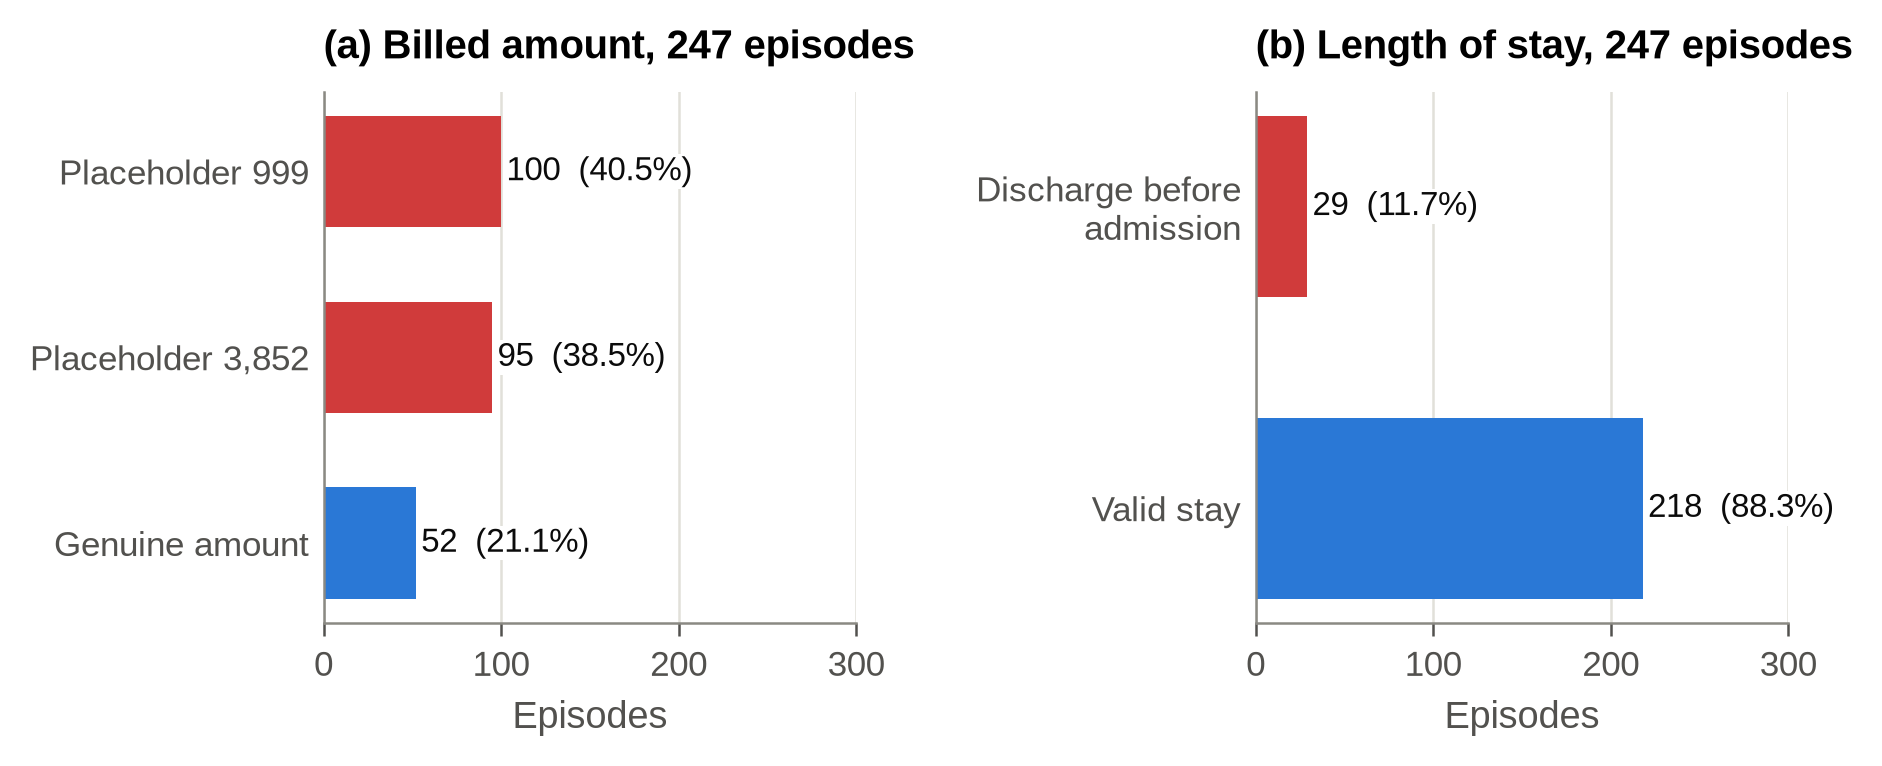
\includegraphics[width=\linewidth]{01_data_quality.png}
\caption{Episodes by billing status (a) and by stay status (b). Defects are shown in
red. Only 52 of the 247 bills are genuine, and 29 stays end before they begin.}
\end{figure}

The flags recomputed from the primary columns agree exactly with the helper columns
supplied with the file (\F{BillIsPlaceholder}, \F{DateError}, \F{LengthOfStay}),
so both defects are confirmed by two independent routes.

% =====================================================================
\section{Cleaning}

\begin{table}[H]\centering\singlespacing
\caption{One decision per problem, with the reason for it}
\small
\begin{tabularx}{\linewidth}{@{}p{3.3cm}r X@{}}
\toprule
\textbf{Problem} & \textbf{Count} & \textbf{Decision and reason} \\ \midrule
Placeholder bills & 195 & Flagged, not deleted. The rows carry a valid diagnosis,
physician, severity and cover; deleting them would discard the clinical record to
repair one column. \F{Bill_clean} holds the amount only where it is genuine. \\
Impossible stays & 29 & \F{LOS_valid} left empty, not set to zero. Zero denotes a
same-day discharge, a real clinical event; writing it would invent 29 of them. \\
Insurance labels & 3 & Mapped to Private, Government and Uninsured, as stable keys for
the dashboard filters. \\
Duplicates & 0 & None removed: identifiers are unique. \\
\bottomrule
\end{tabularx}
\end{table}

Every affected row keeps its flag, so a reader can include or exclude it and see the
difference. \textbf{No row was deleted}: the clean file has the same 247 rows as the
raw file.

% =====================================================================
\section{Indicators}

\begin{table}[H]\centering\singlespacing
\caption{Each indicator with the population it is computed on}
\small
\begin{tabular}{@{}lrl@{}}
\toprule
\textbf{Indicator} & \textbf{Value} & \textbf{Computed on} \\ \midrule
Admission episodes & 247 & all episodes \\
Distinct patients & 75 & all episodes \\
Attending physicians & 7 & all episodes \\
Distinct diagnoses & 10 & all episodes \\
Mean patient age & 47.4 years & all episodes \\
Female share & 52.6\% & all episodes \\
High severity share & 36.0\% & all episodes \\
Uninsured share & 29.1\% & all episodes \\ \midrule
Mean length of stay & 6.74 days & 218 valid stays \\
Median length of stay & 4 days & 218 valid stays \\ \midrule
Validated revenue & 153{,}155 & 52 genuine bills \\
Mean validated bill & 2{,}945 & 52 genuine bills \\
Median validated bill & 2{,}704 & 52 genuine bills \\ \midrule
Raw bill column sum & 618{,}995 & not for decisions \\
\bottomrule
\end{tabular}
\end{table}

Three indicators name their own base. Revenue and the mean bill rest on 52 episodes;
length of stay rests on 218. Naming the base beside the number is better than a
footnote, because a footnote does not travel when a figure is copied into a slide.

\begin{figure}[H]\centering
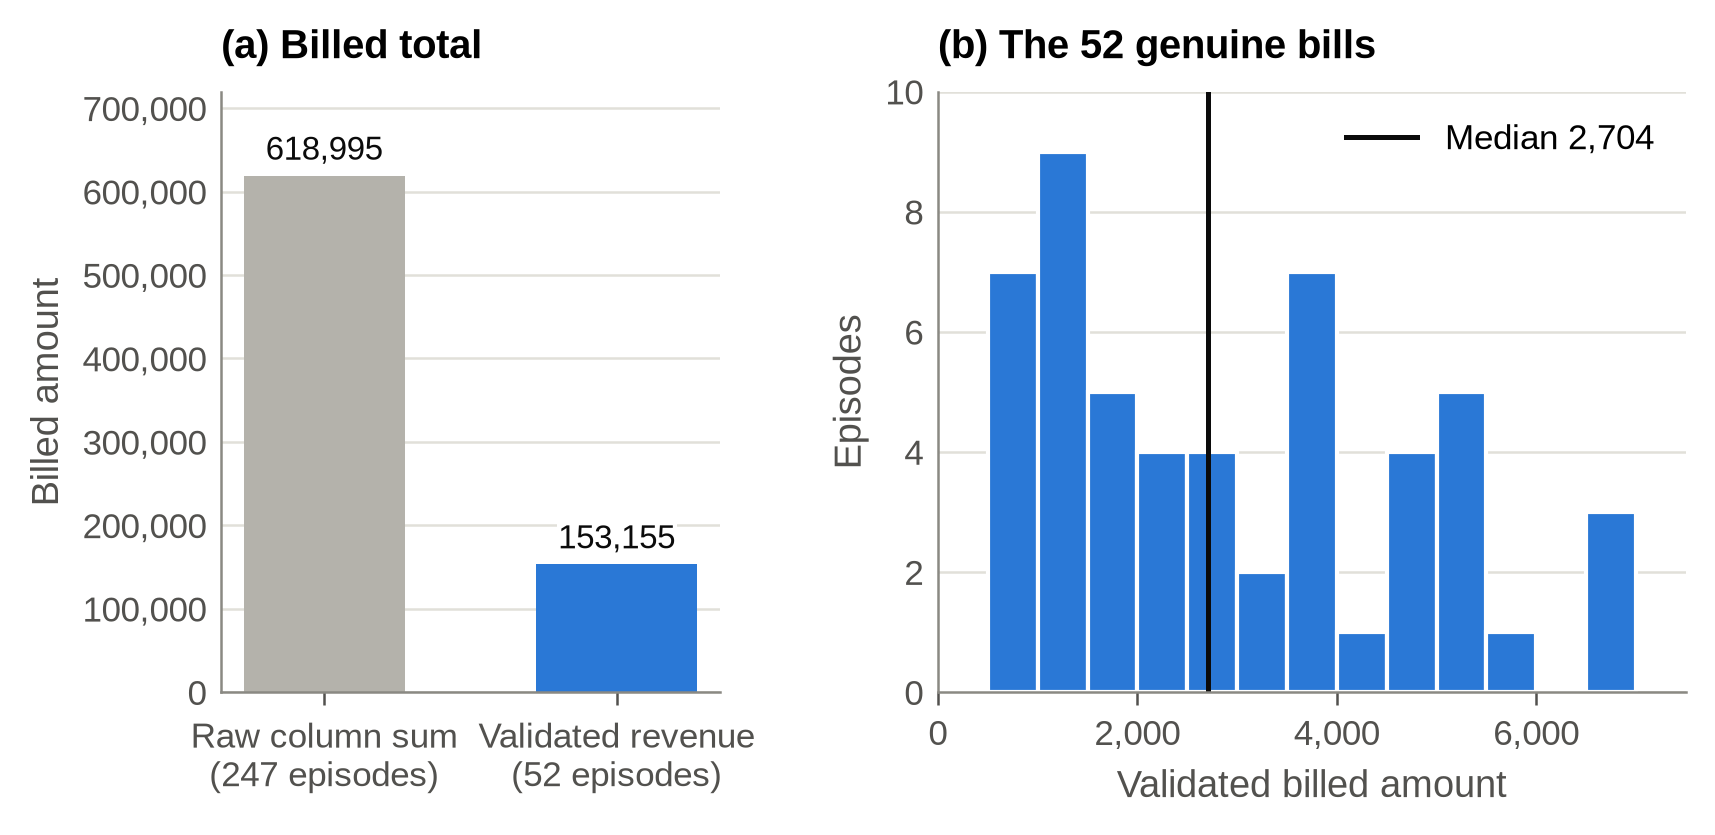
\includegraphics[width=\linewidth]{02_revenue_gap.png}
\caption{Raw bill column sum against validated revenue (a), and distribution of the
52 genuine bills in bins of 500 (b). 465{,}840 of the raw total rests on placeholder
amounts. The genuine bills range from 503 to 6{,}763, with a median of 2{,}704.}
\end{figure}

% =====================================================================
\section{Results}

\subsection{Case mix}

\begin{figure}[H]\centering
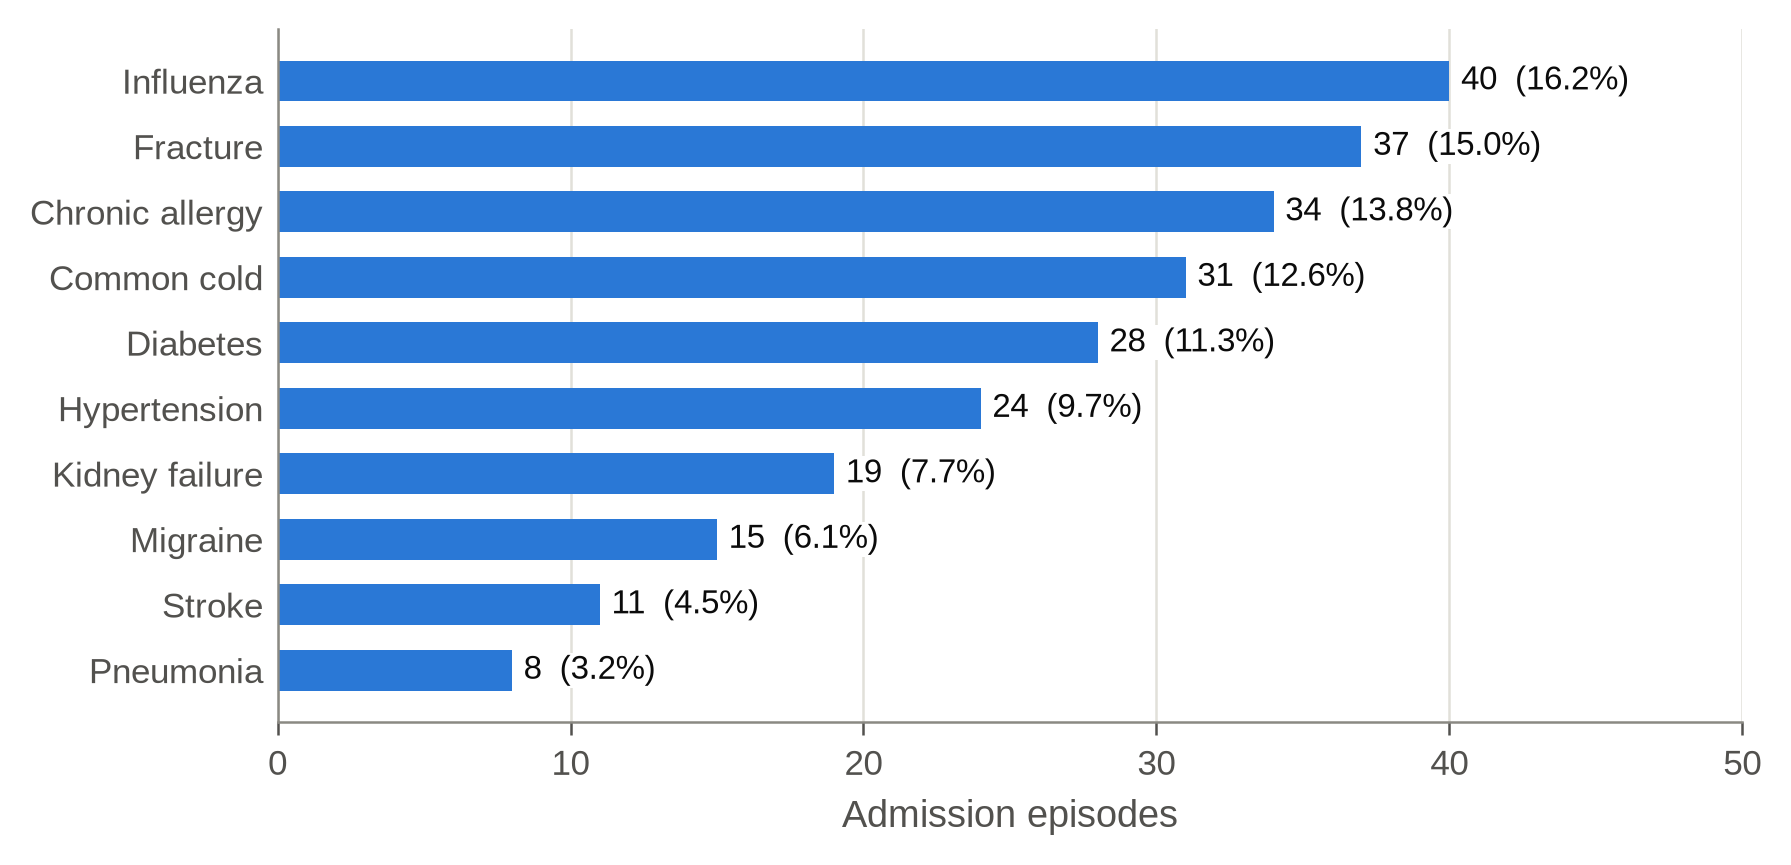
\includegraphics[width=\linewidth]{03_case_mix.png}
\caption{Admission episodes by diagnosis. Influenza (40), fracture (37) and chronic
allergy (34) account for 45\% of admissions.}
\end{figure}

\begin{figure}[H]\centering
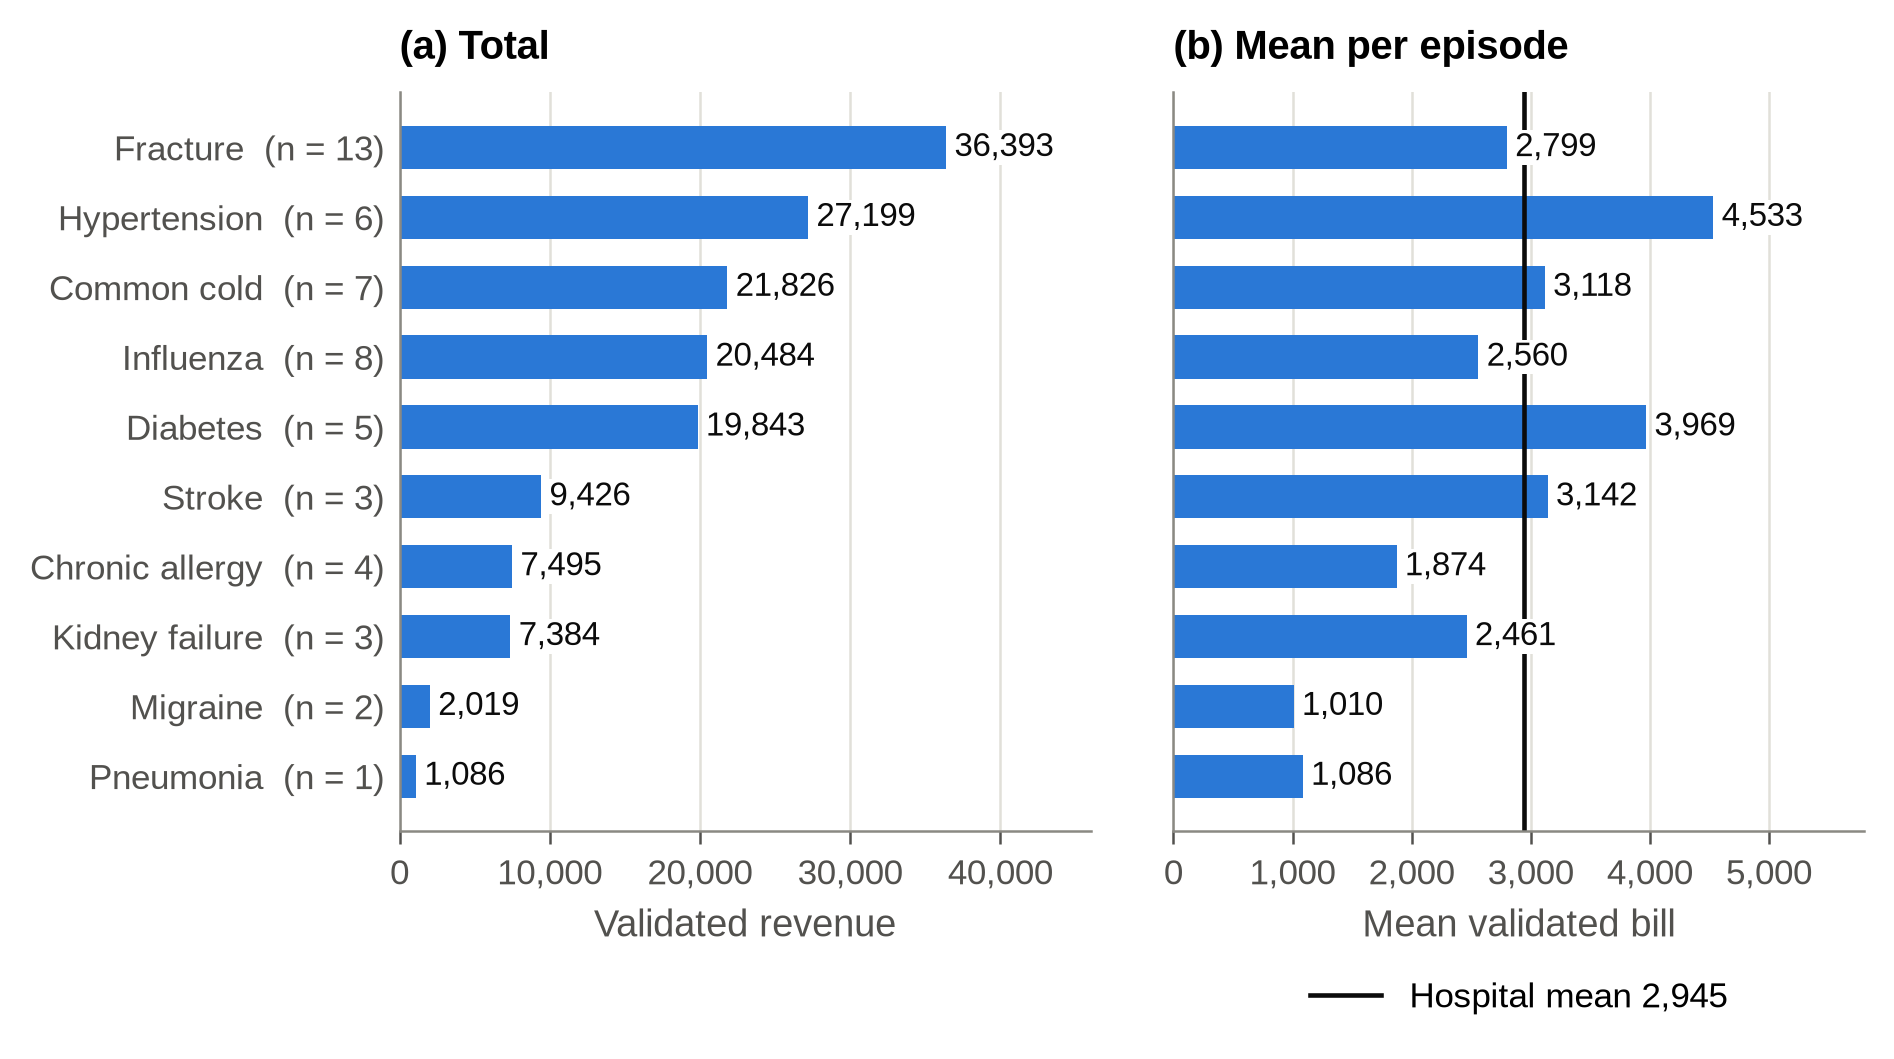
\includegraphics[width=\linewidth]{04_validated_revenue.png}
\caption{Validated revenue by diagnosis: total (a) and mean per episode (b), in the
same diagnosis order. The number of genuine bills is given beside each diagnosis.
Fracture leads total revenue on 13 bills; the highest means, hypertension (4{,}533)
and diabetes (3{,}969), rest on 6 and 5 bills and are indicative only.}
\end{figure}

\subsection{Activity through the year}

\begin{figure}[H]\centering
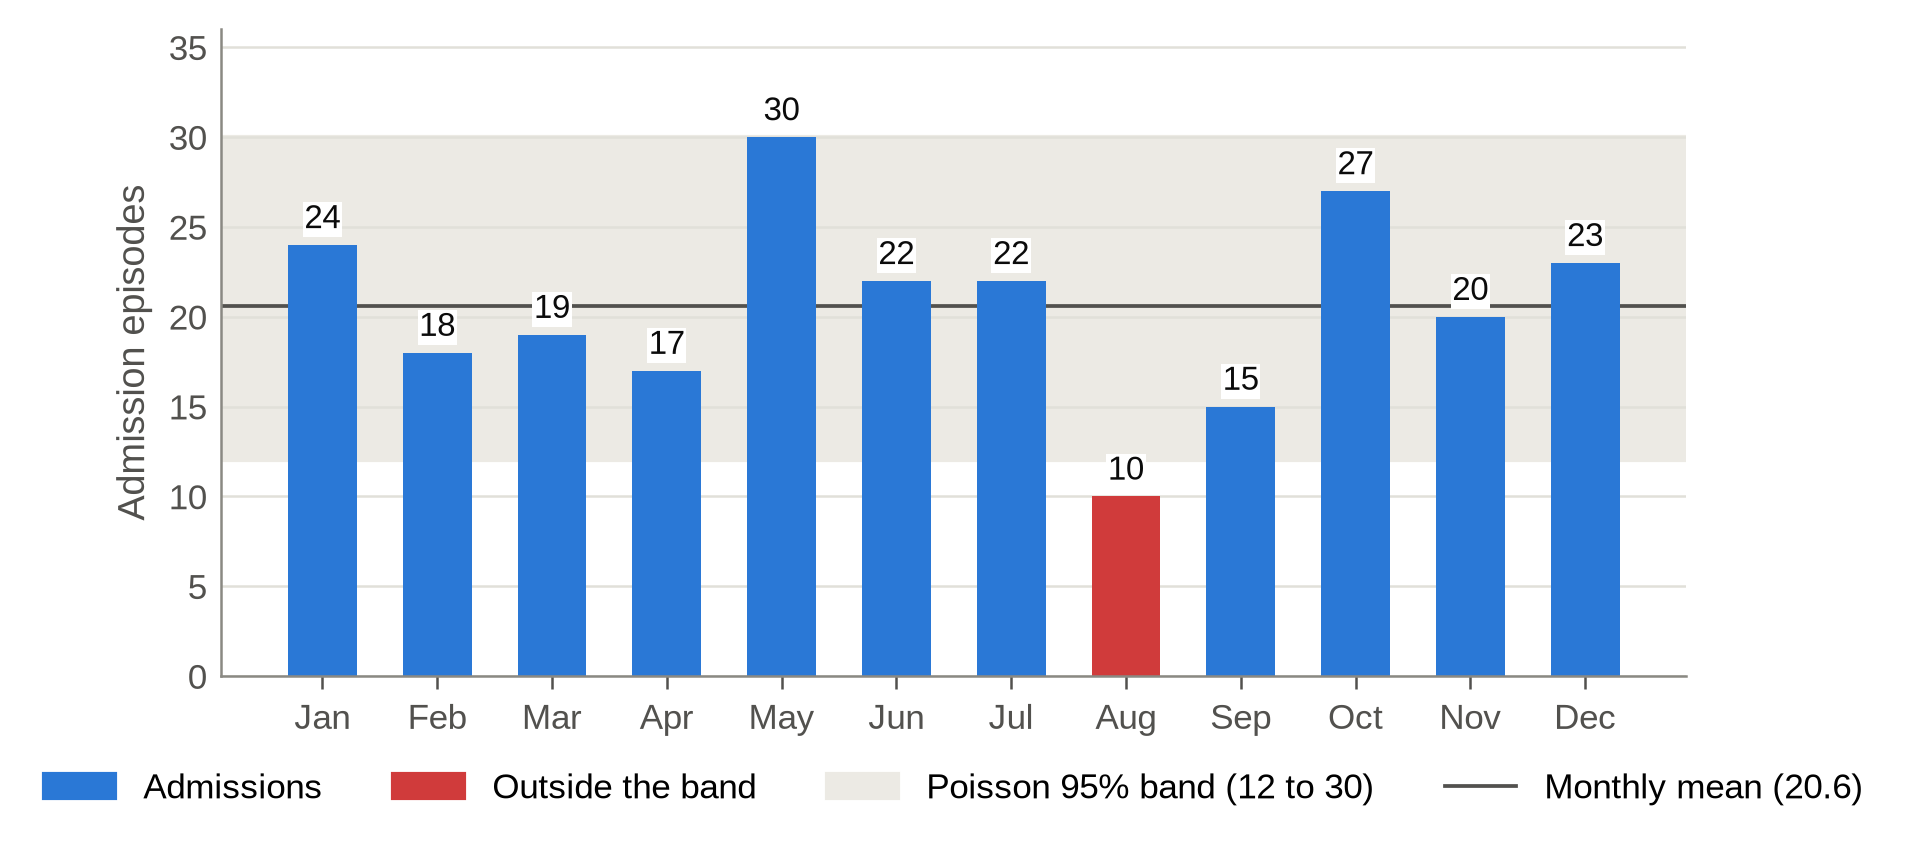
\includegraphics[width=\linewidth]{05_monthly_admissions.png}
\caption{Monthly admissions against the central 95\% range of a Poisson count with
the observed mean (20.6 per month). Only August (10) falls outside the band, about
what chance alone produces over twelve months (0.6 expected). May (30) sits on the
upper edge of the band. A chi-square test does not reject an even spread across
months ($p = 0.17$).}
\end{figure}

\begin{figure}[H]\centering
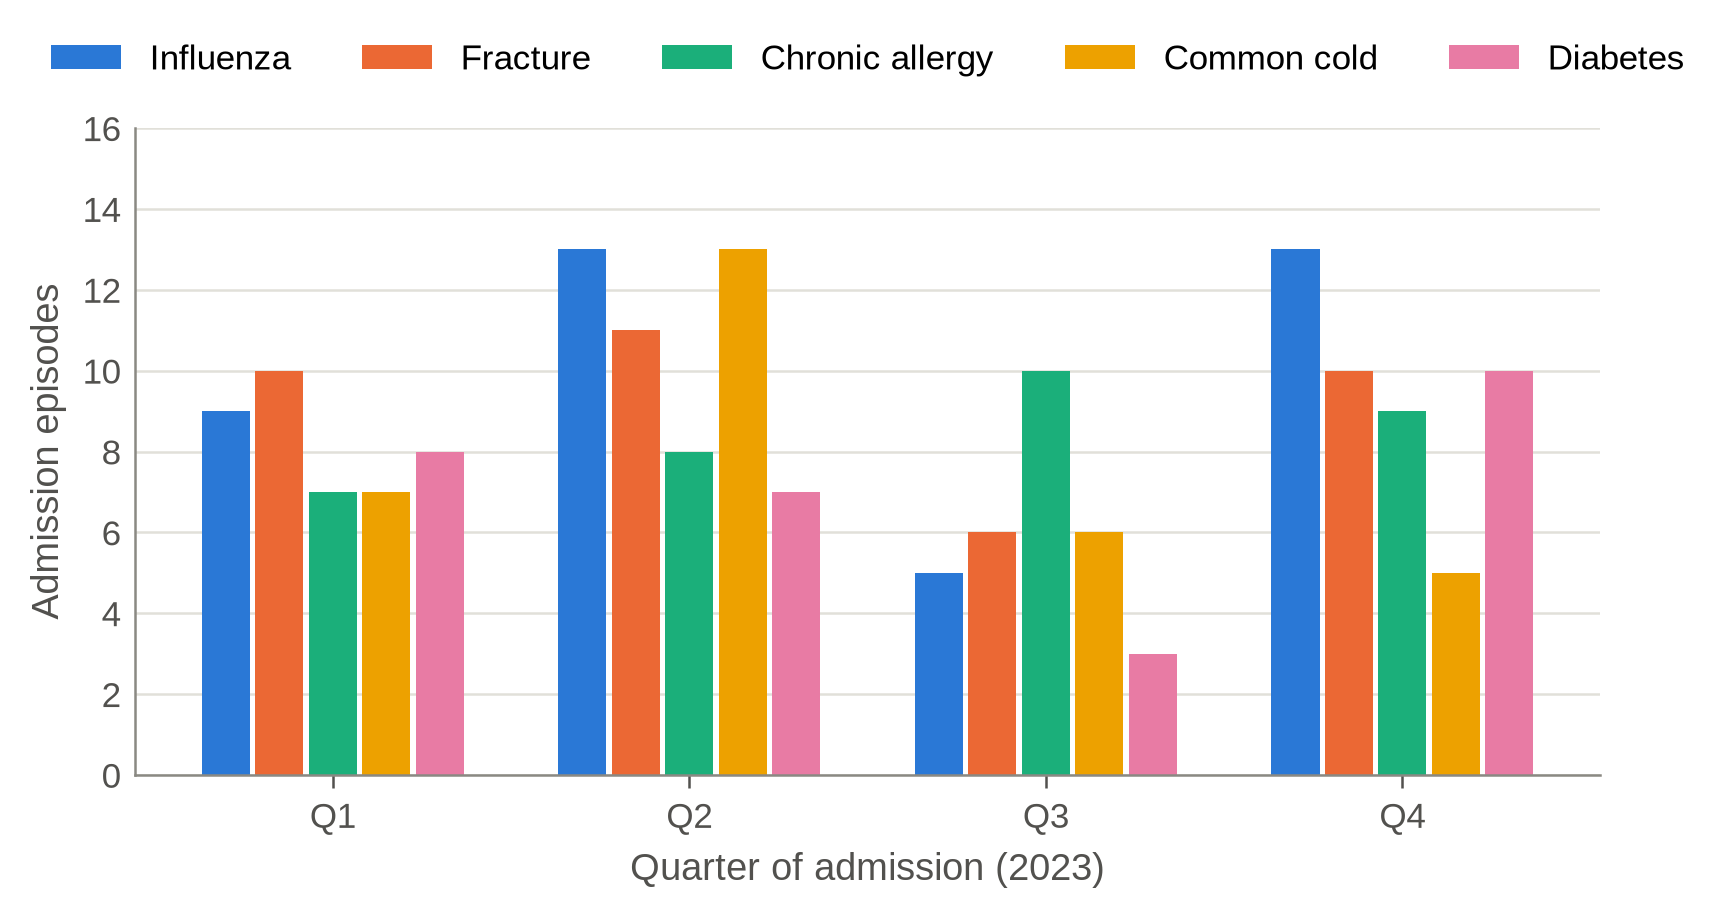
\includegraphics[width=\linewidth]{06_diagnosis_by_quarter.png}
\caption{Quarterly admissions for the five leading diagnoses. The counts are given in
Table~\ref{tab:quarter}.}
\end{figure}

\begin{table}[H]\centering\singlespacing
\caption{Admissions by quarter for the five leading diagnoses}\label{tab:quarter}
\small
\begin{tabular}{@{}lrrrrr@{}}
\toprule
\textbf{Diagnosis} & \textbf{Q1} & \textbf{Q2} & \textbf{Q3} & \textbf{Q4} & \textbf{Year} \\ \midrule
Influenza & 9 & 13 & 5 & 13 & 40 \\
Fracture & 10 & 11 & 6 & 10 & 37 \\
Chronic allergy & 7 & 8 & 10 & 9 & 34 \\
Common cold & 7 & 13 & 6 & 5 & 31 \\
Diabetes & 8 & 7 & 3 & 10 & 28 \\ \midrule
All diagnoses & 61 & 69 & 47 & 70 & 247 \\
\bottomrule
\end{tabular}
\end{table}

\subsection{Acuity, cover and physicians}

\begin{figure}[H]\centering
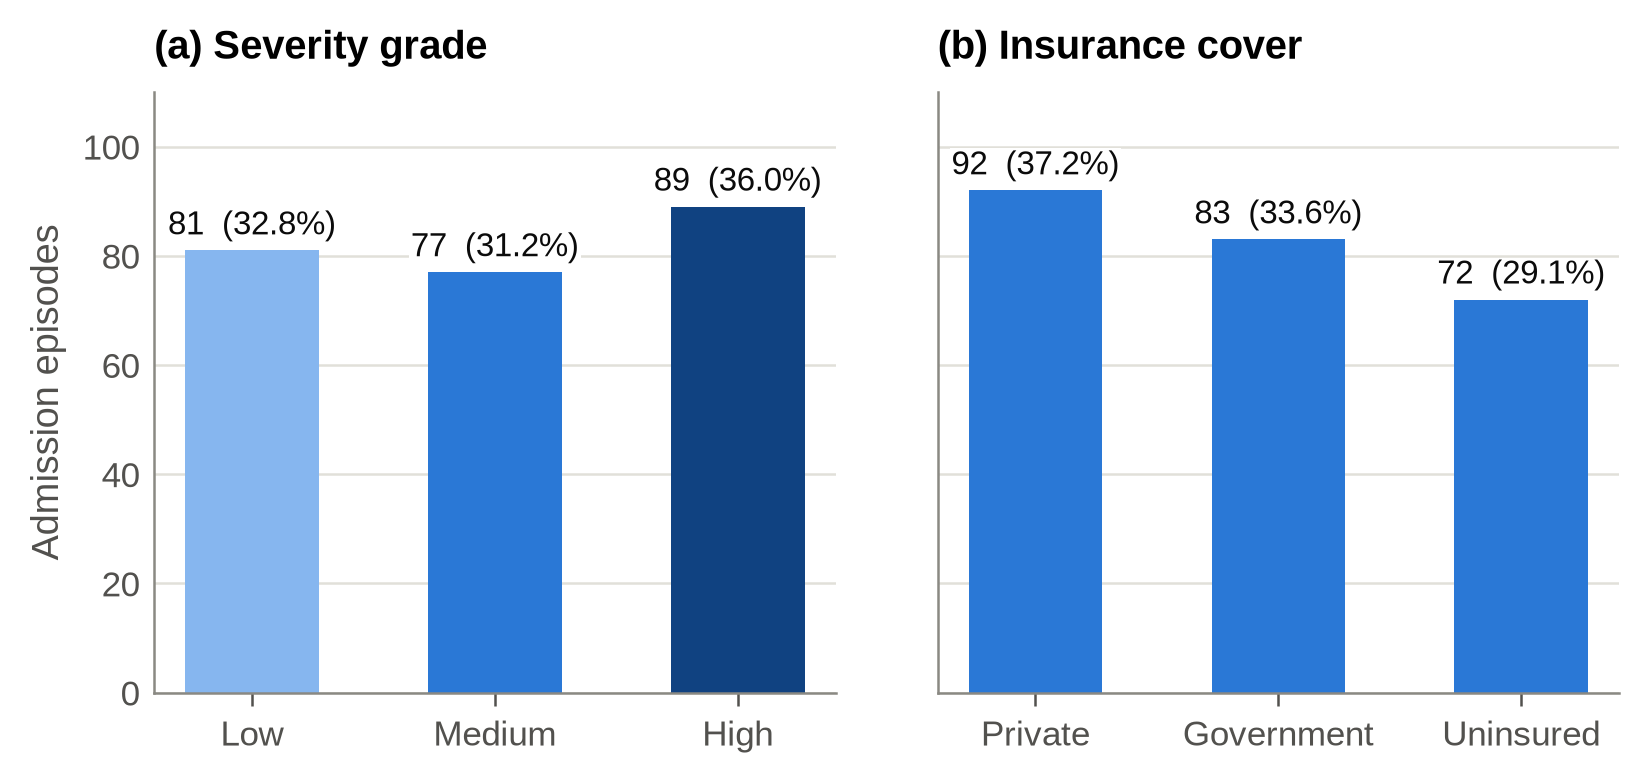
\includegraphics[width=\linewidth]{07_severity_insurance.png}
\caption{Admissions by severity grade (a) and by insurance cover (b). 36.0\% of
admissions are graded high severity and 29.1\% arrive uninsured.}
\end{figure}

\begin{figure}[H]\centering
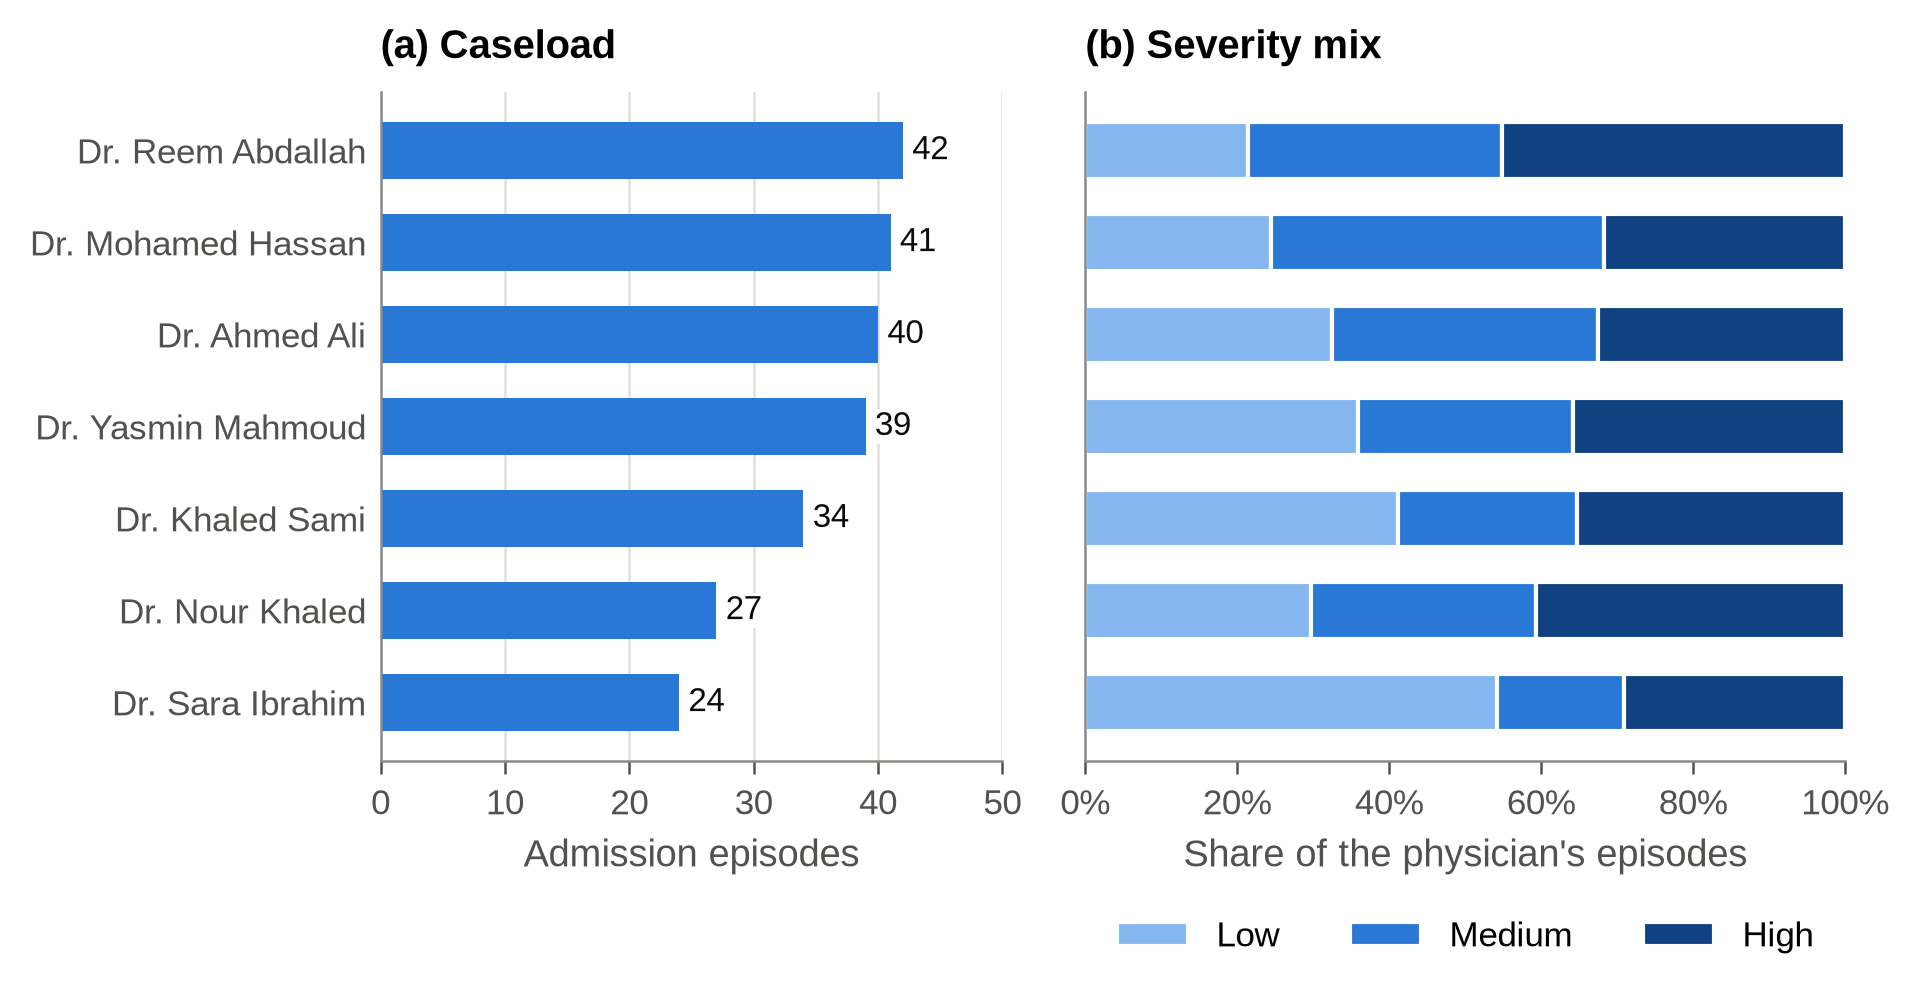
\includegraphics[width=\linewidth]{08_physicians.png}
\caption{Caseload by physician (a) and severity mix of each caseload (b). Caseloads
range from 24 to 42 episodes. The severity mix does not differ significantly between
physicians ($\chi^2 = 13.4$, 12 df, $p = 0.34$): a ranking on this sample would
judge noise.}
\end{figure}

\subsection{Stay, bill and what drives them}

\begin{figure}[H]\centering
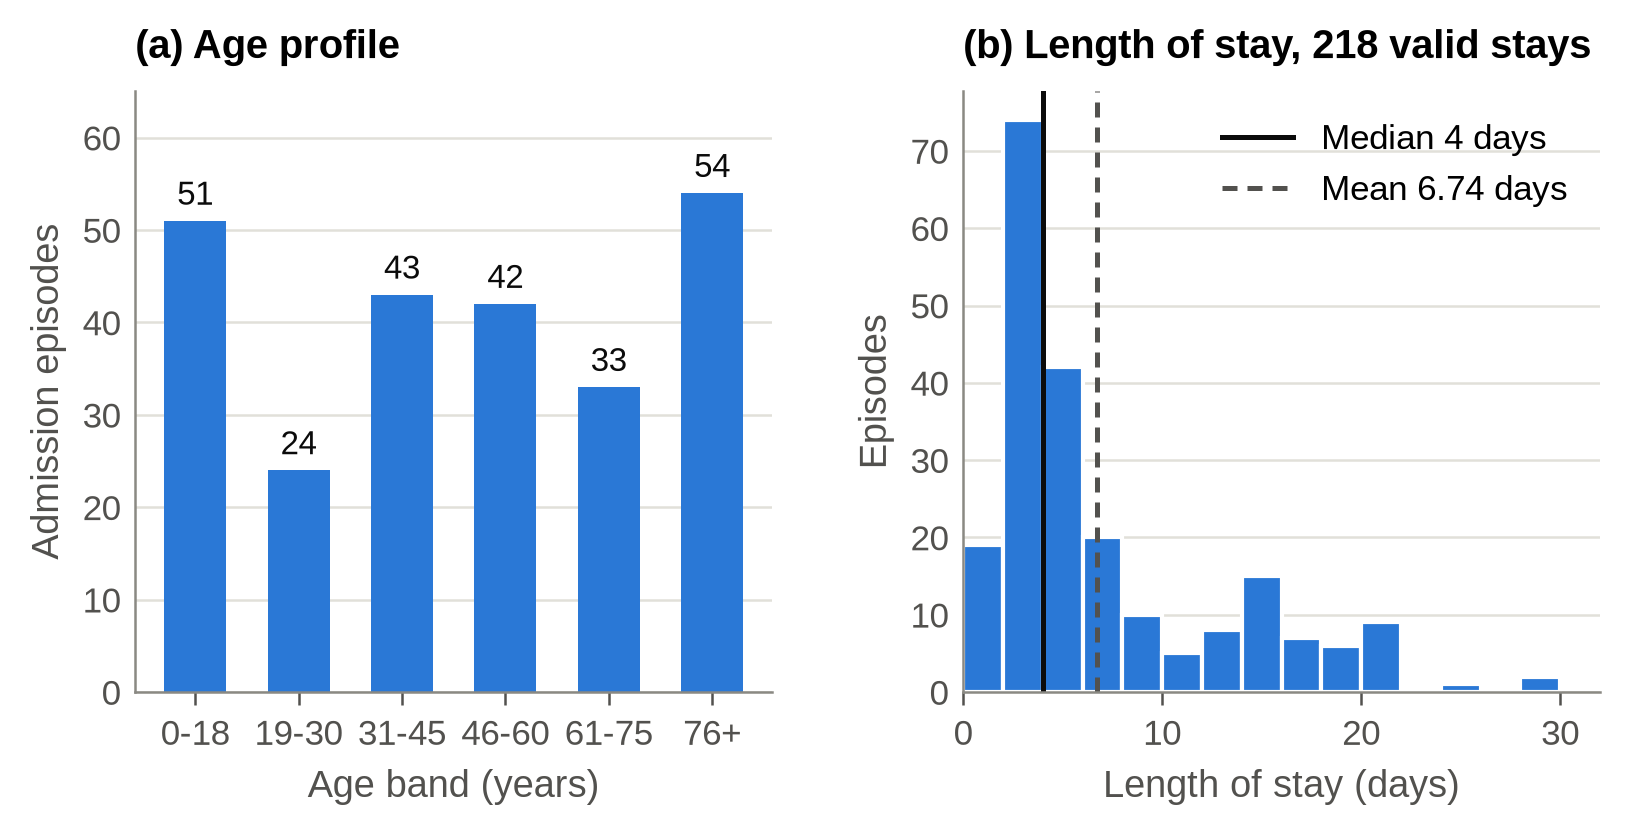
\includegraphics[width=\linewidth]{09_age_los.png}
\caption{Admissions by age band (a) and distribution of the 218 valid stays in bins
of two days (b). The stay distribution is right-skewed: the mean (6.74 days) exceeds
the median (4 days), and 24\% of stays exceed 9 days.}
\end{figure}

\begin{figure}[H]\centering
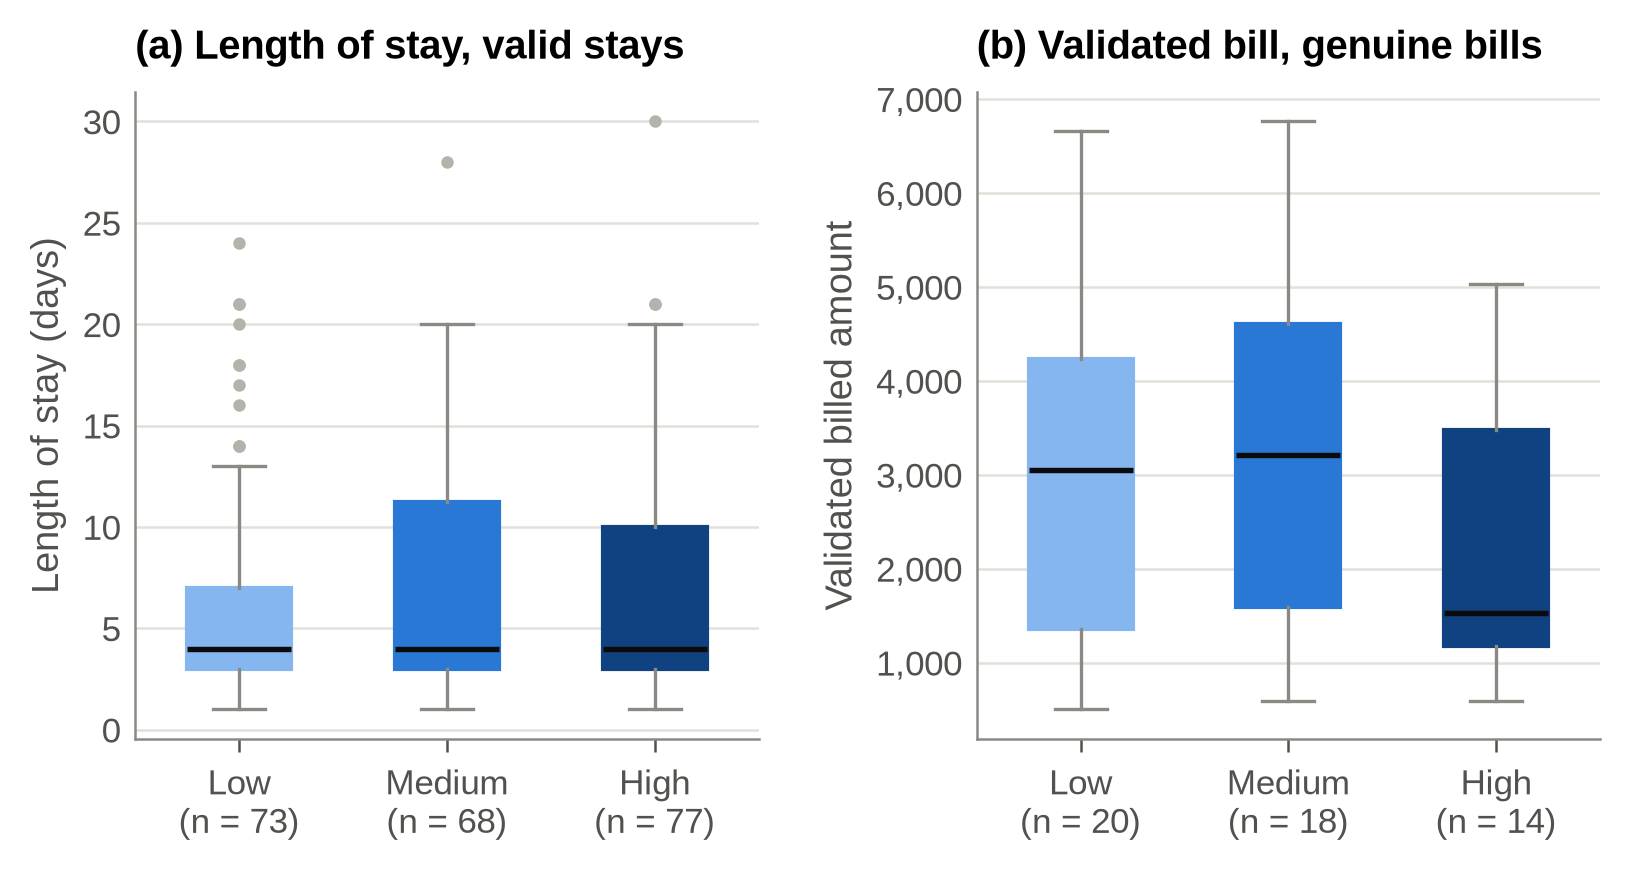
\includegraphics[width=\linewidth]{10_severity_outcomes.png}
\caption{Length of stay (a) and validated bill (b) by severity grade. Boxes show the
interquartile range, black lines the median, whiskers 1.5 times the interquartile
range. The median stay is 4 days in all three grades (Kruskal--Wallis $p = 0.84$);
the bill does not differ either ($p = 0.28$).}
\end{figure}

\begin{figure}[H]\centering
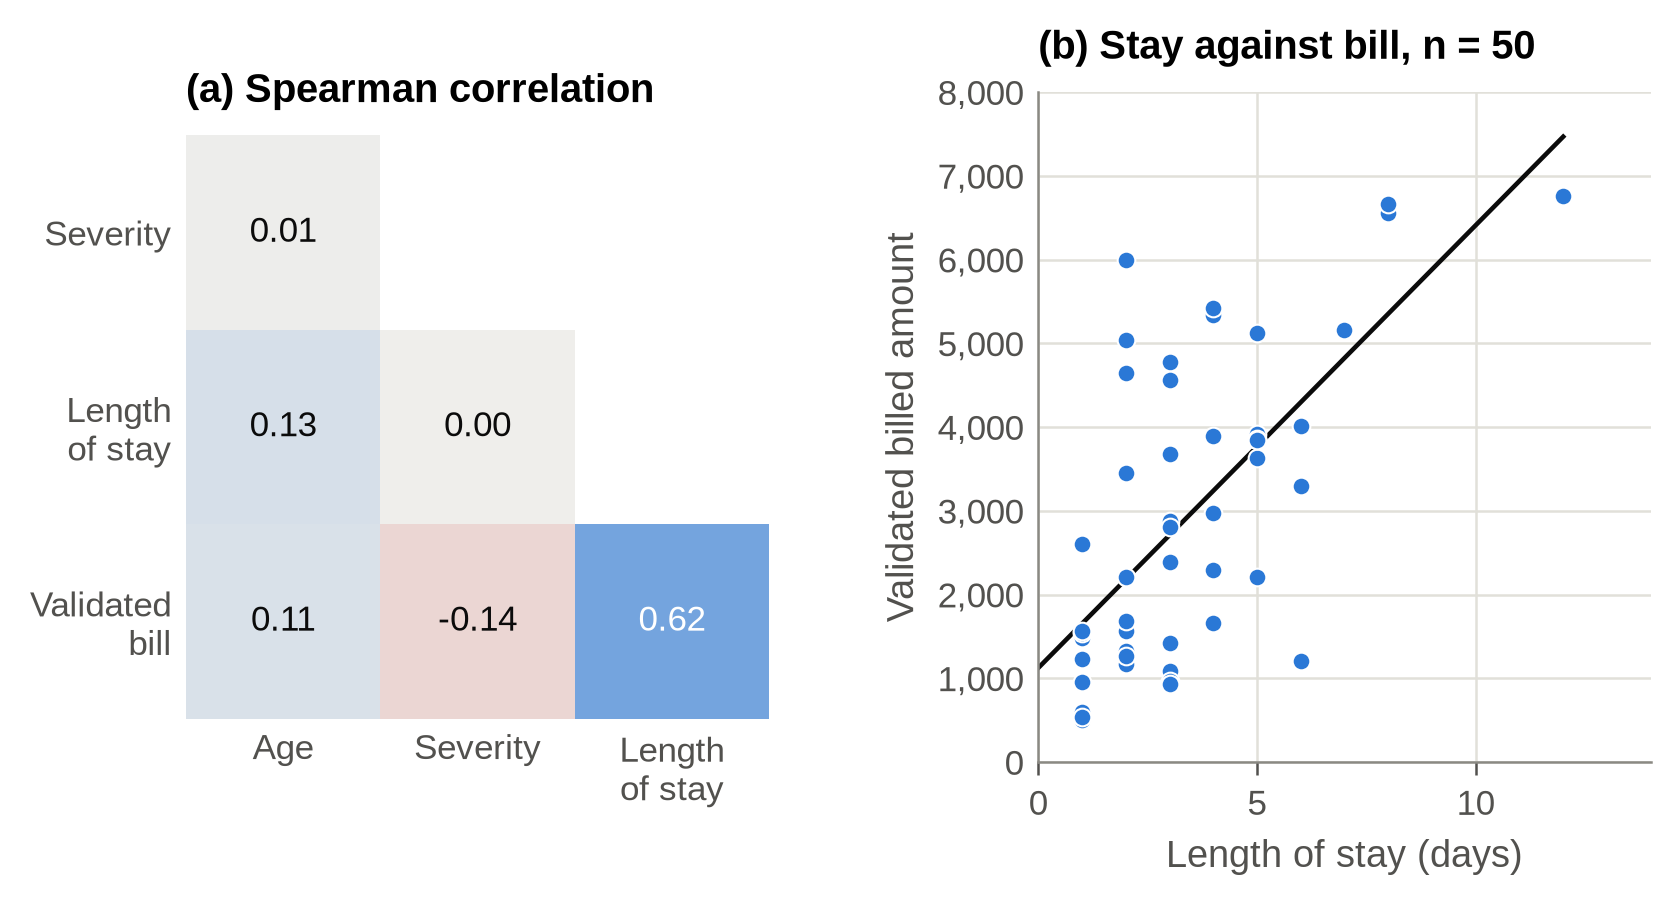
\includegraphics[width=\linewidth]{11_correlations.png}
\caption{Spearman rank correlations between the four numeric measures, each on the
episodes where both values are valid (a), and validated bill against length of stay
for the 50 episodes with both (b). The line is the least-squares fit,
bill $= 1{,}123 + 529 \times$ days. Length of stay is the only measure associated
with the bill ($\rho = 0.62$, $p < 0.001$).}
\end{figure}

\subsection{Representativeness of the genuine bills}

\begin{figure}[H]\centering
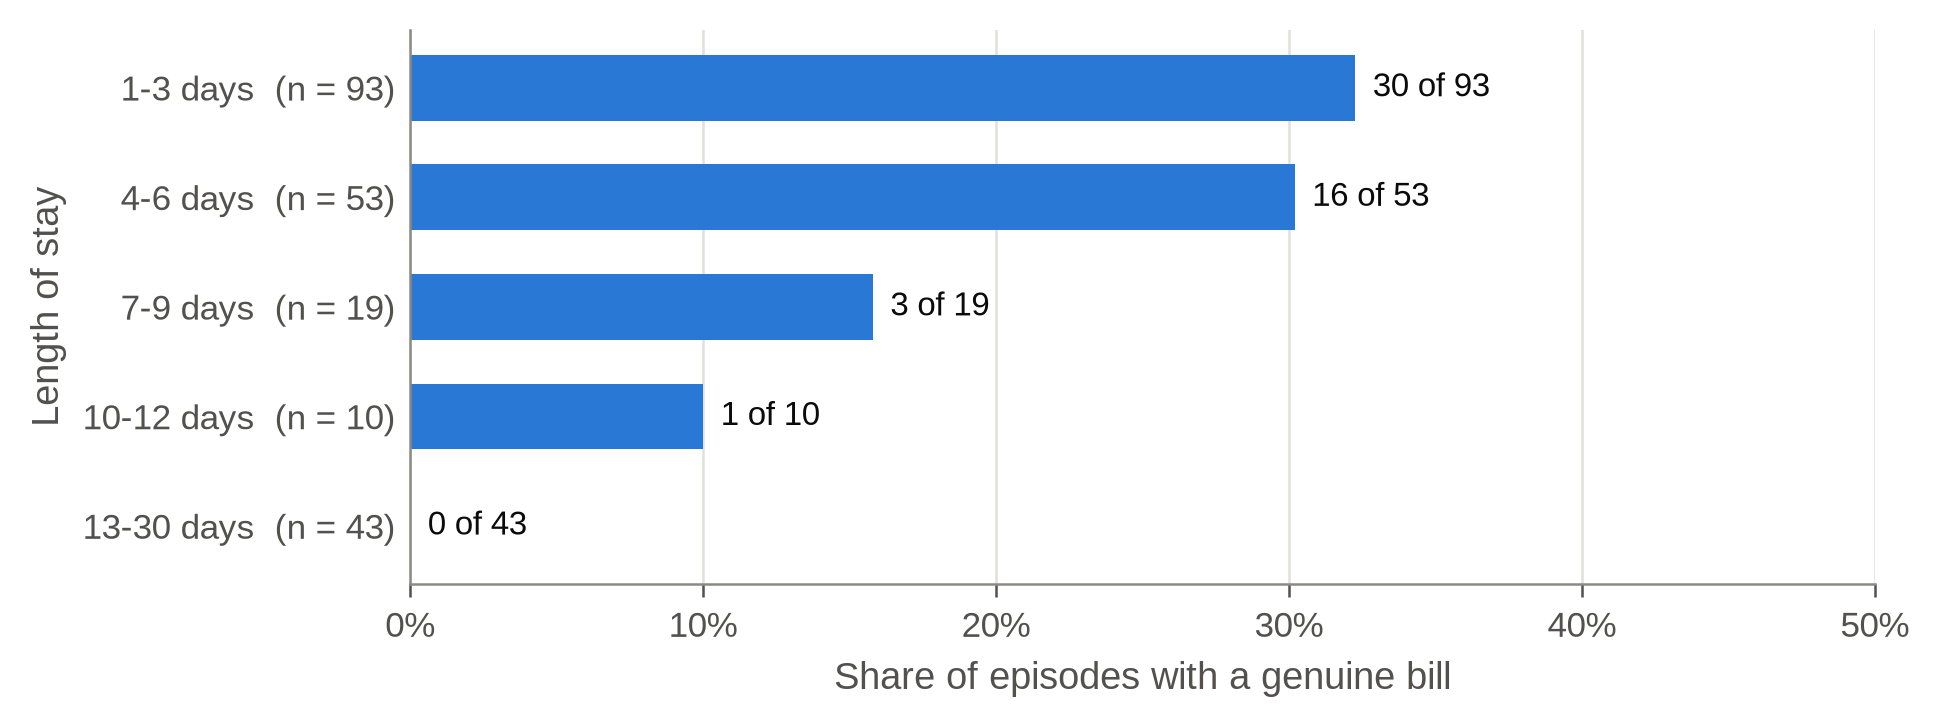
\includegraphics[width=\linewidth]{12_genuine_bills_by_stay.png}
\caption{Share of episodes with a genuine bill, by length-of-stay band. The share
falls from 32\% for stays of 1 to 3 days to 0\% for the 43 stays of 13 days or more.
Genuine bills sit on shorter stays than placeholder bills (median 3 against 5 days,
Mann--Whitney $p < 0.001$).}
\end{figure}

This result governs how every financial figure in this report must be read. The 52
genuine bills are not a random sample of the 247 episodes: they come from short
stays, and the bill rises with the stay. Their mean therefore understates the typical
bill, and multiplying it by 247 would not estimate annual revenue.

% =====================================================================
\section{Statistical tests}

\begin{table}[H]\centering\singlespacing
\caption{Tests behind every segment statement of this report}
\small
\begin{tabular}{@{}llrrr@{}}
\toprule
\textbf{Question} & \textbf{Test} & \textbf{Statistic} & \textbf{$p$} & \textbf{$n$} \\ \midrule
Stay differs by severity & Kruskal--Wallis $H$ & 0.35 & 0.841 & 218 \\
Bill differs by severity & Kruskal--Wallis $H$ & 2.51 & 0.285 & 52 \\
Severity mix differs by physician & $\chi^2$ (12 df) & 13.40 & 0.341 & 247 \\
Severity mix differs by cover & $\chi^2$ (4 df) & 1.19 & 0.880 & 247 \\
Admissions differ by month & $\chi^2$ (11 df) & 15.40 & 0.165 & 247 \\
Stay associated with bill & Spearman $\rho$ & 0.62 & $<0.001$ & 50 \\
Genuine bills on shorter stays & Mann--Whitney $U$ & 2{,}458 & $<0.001$ & 218 \\
\bottomrule
\end{tabular}
\end{table}

Two results are significant at the 5\% level, and both concern the bill: it follows
the length of stay, and the genuine bills over-represent short stays. None of the
segment differences by severity, physician, cover or month is significant.

% =====================================================================
\section{Insights and recommendations}

\subsection{Billing integrity is the primary risk}

195 of 247 episodes carry a placeholder amount. Validated revenue is 153{,}155
against a raw column sum of 618{,}995. The 52 genuine bills also over-represent short
stays, so validated revenue is a floor rather than an estimate.

\textbf{Recommendation.} Publish finance indicators on validated bills only, state
the 52-episode base beside every amount, and do not extrapolate them. Audit the
charge-capture path that writes 999 and 3{,}852 before the next reporting cycle,
starting with long stays, where no genuine bill exists. \emph{Owner: finance and
billing IT.}

\subsection{Date errors break the stay benchmark}

29 episodes record an impossible stay. Mean length of stay on the 218 valid stays is
6.74 days, median 4 days.

\textbf{Recommendation.} Block the save when the discharge date precedes the
admission date. One validation rule at entry would have preserved 11.7\% of the
year's operational record. \emph{Owner: admission system IT.}

\subsection{Length of stay, not severity, drives the bill}

The bill rises by about 530 per day of stay over the 1 to 12 days observed. Severity
predicts neither the stay nor the bill, and medium-severity stays are as long as
high-severity ones.

\textbf{Recommendation.} Manage cost through discharge planning for long stays: one
valid stay in four exceeds 9 days. Audit how the severity grade is assigned at
admission; a triage grade that predicts neither stay nor bill needs correcting.
\emph{Owner: medical direction.}

\subsection{Case mix is concentrated; acuity and cover create pressure together}

Influenza, fracture and chronic allergy account for 45\% of admissions. 36.0\% of
admissions are graded high severity and 29.1\% arrive uninsured.

\textbf{Recommendation.} Align bed, pharmacy and pathway capacity with the three
leading diagnoses. Move financial counselling for uninsured patients to admission
rather than discharge. \emph{Owner: operations and patient services.}

\subsection{The monthly profile does not support a seasonal roster}

Admissions are compatible with an even spread across the year ($p = 0.17$). Only
August falls outside the range chance produces.

\textbf{Recommendation.} Do not build a staffing roster on the shape of a single
year. Re-test seasonality when a second year is available. \emph{Owner: operations.}

% =====================================================================
\section{The interactive dashboard}

\F{dashboard.html} is a single self-contained file: no server and no installation.
It is built with Python and Plotly. The left navigation bar opens seven views:
Overview, Dashboard, Patients, Clinical, Financial, Data Quality and Insights. Key
indicators, charts and tables are rendered in the browser, and filters on month,
physician, diagnosis, insurance, gender and severity update every visual at once.
A live-data dock reloads a cleaned CSV or Excel file and recomputes the indicators,
charts, correlations and insights.

An optional WebSocket server, \F{websocket_server.py}, streams the indicators from the
clean register to the dashboard and follows its filters (\F{WEBSOCKET.md} documents
the protocol). It computes revenue on genuine bills and length of stay on valid stays,
so a streamed figure always matches this report. The dashboard works without it.

\subsection{Reading the dashboard against this report}

Three dashboard elements use a different base from the report. They are listed here
so that no reader meets an unexplained difference.

\begin{table}[H]\centering\singlespacing
\caption{Reconciliation between dashboard elements and report indicators}
\small
\begin{tabularx}{\linewidth}{@{}p{4.6cm}X@{}}
\toprule
\textbf{Dashboard element} & \textbf{Base used and report equivalent} \\ \midrule
\emph{Revenue} tile (618{,}995); \emph{Revenue by insurance}, \emph{Revenue by
diagnosis}, \emph{Revenue trend} & Raw bill column, placeholders included.
Report equivalent: validated revenue, 153{,}155 (Financial view,
\emph{Validated revenue} tile). \\
\emph{Avg bill} tile (2{,}506) & Raw bill column divided by 247 episodes. Report
equivalent: mean validated bill, 2{,}945 on 52 genuine bills. \\
\emph{Billing quality} alert (100 placeholder bills) and \emph{Clinical correlations}
cards & Only 999 treated as a placeholder; the 95 bills at 3{,}852 are kept. Report
equivalent: 195 placeholder bills; stay--bill Pearson $r = 0.66$ on 50 genuine bills
(the card shows 0.31 on 133 episodes). \\
\bottomrule
\end{tabularx}
\end{table}

All other dashboard values (volumes, case mix, severity, cover, length of stay, data
quality counts) are identical to the report. The captures below were taken with every
filter cleared.

\subsection{Overview}

\capture{overview_1.png}{Overview, alert bar. Real-time alerts on billing quality,
date quality, acuity, payer risk, long stays, monthly peak and age.}
\capture{overview_2.png}{Overview, headline indicators with admissions by month, top
diagnoses and top physicians.}
\capture{overview_3.png}{Overview, severity and insurance mix with the headline
insights.}
\capture{overview_4.png}{Overview, end of the headline insights: volume and cost by
pathology.}

\subsection{Dashboard}

\capture{dashboard_1.png}{Dashboard, indicator strip and filter bar (month, doctor,
diagnosis, insurance, gender, severity).}
\capture{dashboard_2.png}{Dashboard, admissions and mean length of stay by month, age
groups and gender split.}
\capture{dashboard_3.png}{Dashboard, billed amount by month, top diagnoses and length
of stay by severity.}
\capture{dashboard_4.png}{Dashboard, top physicians, insurance mix and key insights.}

\subsection{Patients}

\capture{patients_1.png}{Patients, the patient explorer: one row per episode with
diagnosis, severity, physician, dates, stay, bill and cover.}
\capture{patients_2.png}{Patients, end of the first page of the explorer, with
pagination over the 247 episodes.}

\subsection{Clinical}

\capture{clinical_1.png}{Clinical, diagnosis mix by quarter.}
\capture{clinical_2.png}{Clinical, diagnosis volume and billed amount by diagnosis.}
\capture{clinical_3.png}{Clinical, physician caseload and severity profile.}

\subsection{Financial}

\capture{financial_1.png}{Financial, total billed, validated revenue and average bill,
with billed amount by insurance and by diagnosis.}

\subsection{Data Quality}

\capture{data_quality.png}{Data Quality, the defect counts: 247 episodes, 29 date
errors, 195 placeholder bills, 7 physicians.}

\subsection{Insights}

\capture{insights_1.png}{Insights, clinical correlation cards.}
\capture{insights_2.png}{Insights, monthly snapshot of admissions, validated revenue
and mean length of stay.}
\capture[0.85\linewidth]{insights_3.png}{Insights, the decision insights.}
\capture[0.85\linewidth]{insights_4.png}{Insights, priorities and the live-data dock for reloading a
cleaned file.}

% =====================================================================
\section{Limitations}

\textbf{Revenue rests on 52 episodes, concentrated on short stays.} No financial
figure in this report is a budget input until the billing column is repaired at
source. Means by diagnosis rest on 1 to 13 bills, and the stay--bill slope is only
observed between 1 and 12 days.

\textbf{Length of stay rests on 218 episodes}, 88.3\% of the file.

\textbf{The sample is small for the number of segments.} 247 episodes across 10
diagnoses and 7 physicians leaves several segments in single figures. Every segment
comparison is reported with its test.

\textbf{One facility, one year.} There is no ward or site column, so no comparison
between units is possible, and a single year supports no trend or seasonality claim.

\textbf{Association, not causation.} The stay--bill relationship shows that the bill
follows the stay; it does not show why stays are long.

% =====================================================================
\section{Reproducibility}

Every number, table and figure of this report is produced by the notebook
\F{MediCare-Hospital-Analytics.ipynb} from the raw file \F{data/hospital_raw.csv}.
The notebook writes the clean register (\F{data/hospital_clean.csv}), the result
tables (\F{results/}) and the figures (\F{figures/}, PNG at 300~dpi). Once
the billing and date capture are repaired at source, re-running the notebook
unchanged recomputes every flag, indicator, test and figure.

\vspace{0.3cm}
\noindent\hfill\begin{minipage}{7cm}\begin{flushright}\singlespacing
\textbf{KOUAME Koffi Fid\`ele}\\
Data Analysis Internship\\
\href{mailto:koffifidelek59@gmail.com}{koffifidelek59@gmail.com}
\end{flushright}\end{minipage}

\end{document}
